
\begin{figure}

\begin{minipage}{0.5\textwidth}
\small
\begin{verbatim}
function visit( Node v ) {
  globals.time++;
  discovery[ v.getId() ] = globals.time;
  beginStep();
  v.setLabel( "" + discovery[ v.getId() ] );
  v.selected( true );
  endStep();
  for_outgoing( v, e, w ) {
    beginStep();
    if ( ! w.isSelected() ) {
      e.setSelected(true);
       visit( w );
    }
    else if ( finish[ w.getId() ] == 0 ) {
      e.setLabel( "B" );  /* ancestor */
    }
    else if ( finish[ w.getId() ]
              > discovery[ v.getId() ] ) {
      e.setLabel( "F" );  /* descendant */
    }
    else {
      e.setLabel( "C" );
    }
    endStep();
  }
  beginStep();
  globals.time++;
  finish[ v.getId() ] = globals.time;
  v.mark();
  v.setLabel( "" + discovery[ v.getId() ]
              + "/" + finish[ v.getId() ] );
  endStep();
}

setDirected( true );

beginStep();
for_nodes( u ) {
    u.setLabel("");
}
for_edges( e ) {
    e.setLabel("");
}
endStep();

for_nodes( u ) {
    if ( ! u.isSelected() ) {
        visit( u, null );
    }
}

\end{verbatim}
\end{minipage}
\begin{minipage}{0.49\textwidth}
\centering

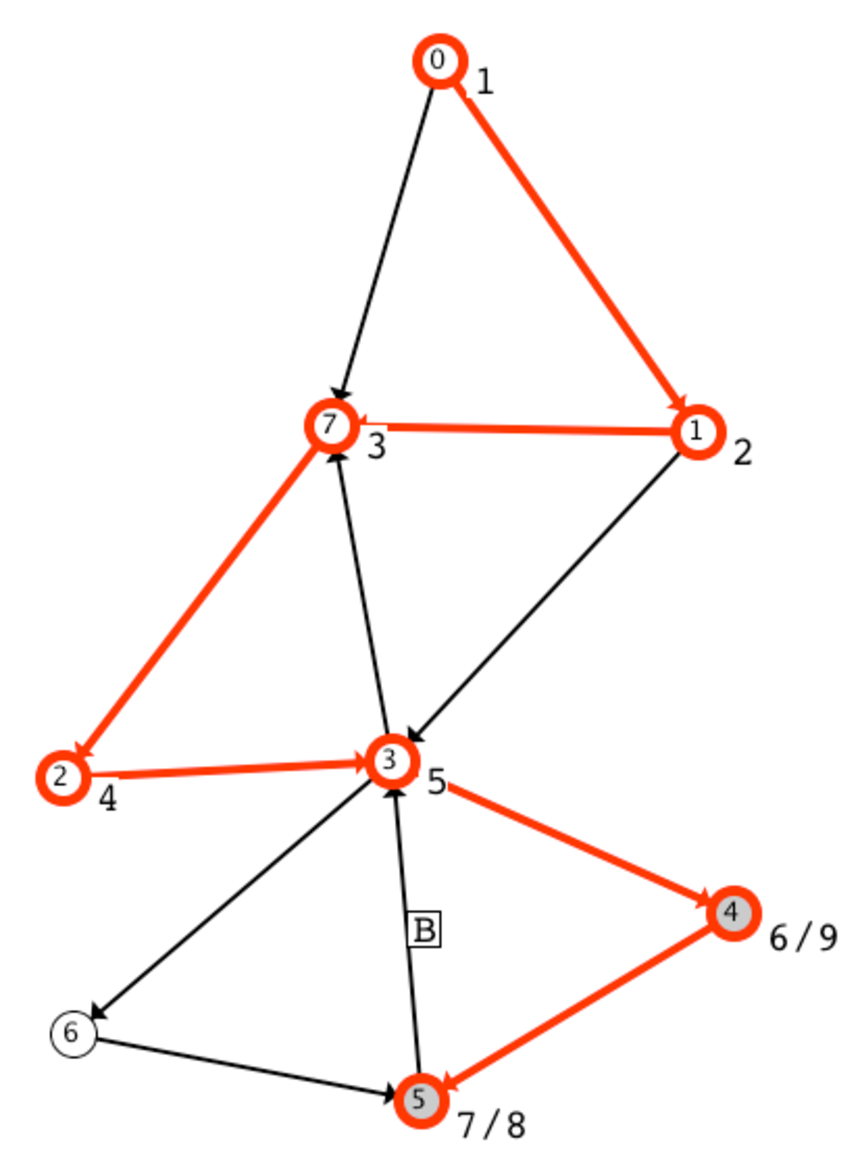
\includegraphics[scale=0.5]{X_dfs_d_1}

After first non-tree edge is labeled. 

\medskip

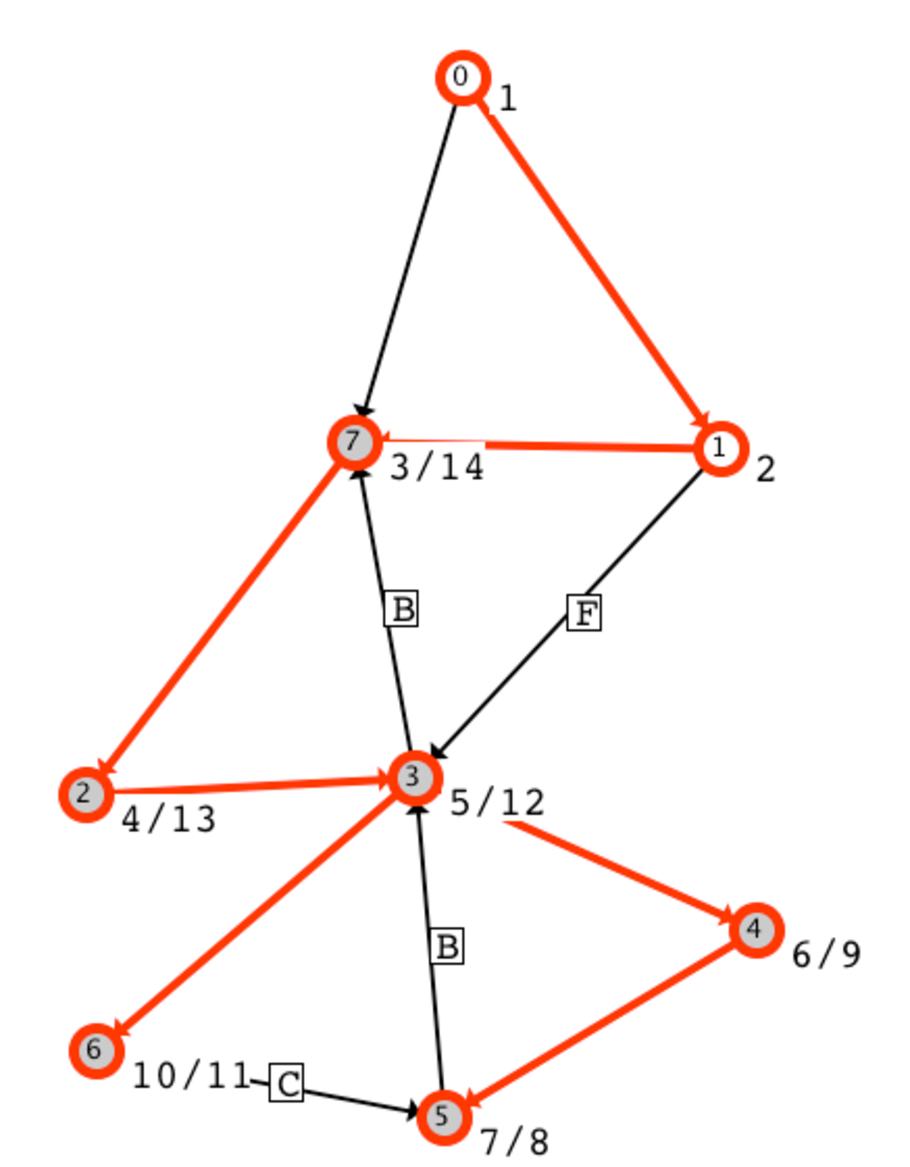
\includegraphics[scale=0.5]{X_dfs_d_2}

After all but one non-tree edges have been labeled.

\end{minipage}
\caption{Implementation of a depth-first search animation
  with an illustration of the graph panel during execution.}
\label{fig:dfs}
\end{figure}
